% ****** Start of file aipsamp.tex ******
\documentclass[%
 aip,
 jmp,%
 amsmath,amssymb,
%preprint,%
 reprint,%
%author-year,%
%author-numerical,%
]{revtex4-2}
\usepackage{subfigure}
\usepackage{graphicx}% Include figure files
\usepackage{dcolumn}% Align table columns on decimal point
\usepackage{bm}% bold math
%\usepackage[mathlines]{lineno}% Enable numbering of text and display math
%\linenumbers\relax % Commence numbering lines

\begin{document}

\preprint{AIP/123-QED}

\title[Catalytic knowledge graph construction and application]{Catalytic knowledge graph construction and application}% Force line breaks with \\
\thanks{Footnote to the title of the article.}

\author{Qingqing Li}
\altaffiliation{Chemistry and Chemical engineering Department, Xiamen University.}%Lines break automatically or can be forced with \\
\email{liqingqing@stu.xmu.edu.cn}

\date{\today}% It is always \today, today,
             %  but any date may be explicitly specified

\begin{abstract}
    The current implementation of relay catalysis, an essential approach for the synthesis of essential chemical feedstocks such as ethanol and formaldehyde, is still heavily reliant on a laborious reading of literature, searching for reactions manually, and time-consuming analysis of reaction pathways. With recent developments in artificial intelligence, it is now possible to automatically gather literature and extract reaction information from it. This paper describes how to collect literature, extract reaction data from the literature, and connect it into the form of a knowledge graph leveraging the relationship that the products of the previous step of the reaction are the reactants of the subsequent step of the reaction.  The scoring rules are designed for the reaction pathways in the knowledge graph, and the better relay catalytic routes are obtained by scoring and ranking the paths for producing specified products, completing the automated system for relay catalytic path screening.
\end{abstract}

\keywords{Knowledge graph, Relay catalysis, Reaction database, Specific-product synthesis pathway selection}
%Use the show keys class option if the keyword
%display desired
\maketitle

% \begin{quotation}
% The ``lead paragraph'' is encapsulated with the \LaTeX\ 
% \verb+quotation+ environment and is formatted as a single paragraph before the first section heading. 
% (The \verb+quotation+ environment reverts to its usual meaning after the first sectioning command.) 
% Note that numbered references are allowed in the lead paragraph.
% %
% The lead paragraph will only be found in an article being prepared for the journal \textit{Chaos}.
% \end{quotation}


\section{Introduction}
% \subsection{Catalytic knowledge}
Catalytic reactions\cite{allen2012synergistic}, which enhance chemical processes by using catalysts, have gained broad preference as a method of lowering a reaction's activation energy, substantially improving reaction efficiency, and drastically reducing energy consumption. The conventional catalytic model\cite{somorjai1986structure} is primarily based on a single catalyst catalyzing a single reaction, followed by a step-by-step linear synthesis to produce the desired product. However, improving the selectivity and conversion of a catalytic reaction in practice is a difficult challenge, and it can be challenging to enhance both simultaneously. Modern organic synthesis advocates more atomic economy\cite{trost1991atom} as well as stepwise economy\cite{zhang2019one}, as demonstrated by Fischer-Tropsch synthesis\cite{anderson1984fischer}, which converts coal into high-carbon compounds and liquid fuels via syngas. Because of the limits of the reaction principle and the ASF model\cite{fortsch2015product}, it is difficult to improve the products' carbon chain length selectivity. To address this issue, Wang Ye and Bao Xinhe developed the relay catalysis strategy\cite{wu2013asymmetric}, which can combine multiple catalysts to achieve a one-pot tandem reaction\cite{csekei2008development}, in which different types of catalysts can synergistically or independently realize the traditional multistep synthesis\cite{webb2010continuous} in a single operation, greatly reducing waste of raw materials, solvents, and time while also improving the efficiency of the reaction. A comparison between the traditional catalytic model and the relay catalytic approach is shown in the figure(Fig.\ref{ Fig.1 }). This strategy can be used to improve the selectivity of high-value-added chemicals by designing multifunctional catalysts\cite{felpin2008heterogeneous} and integrating multistep catalytic reactions into a continuous process to achieve direct and efficient intermediate conversion and improve target product selectivity. However, the development of relay catalysis faces numerous difficulties and challenges, such as the design of relay catalytic pathways and multifunctional catalysts, which is heavily reliant on literature searches and the experience of human experts, making relay catalysis research time-consuming and expensive. As a result, figuring out how to use computer technology to swiftly select appropriate catalysts and reaction circumstances has emerged as a major challenge in the science of catalysis.

\begin{figure}[htbp]
    \centering
    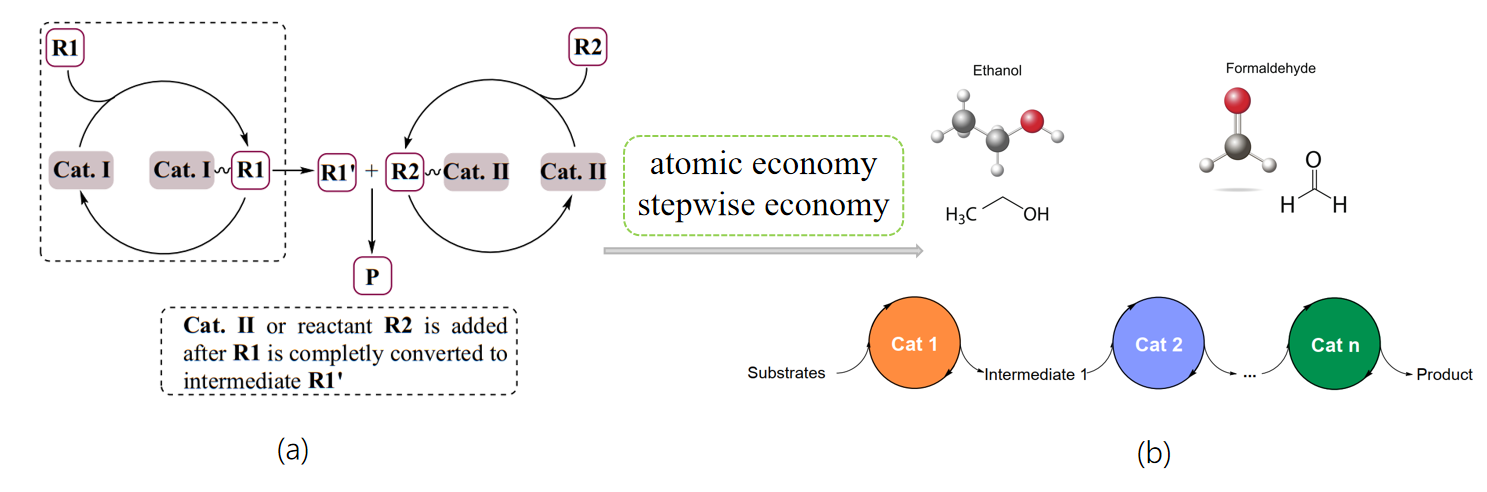
\includegraphics[width=1\textwidth]{figure/1.png}
    \caption{ (a). Traditional catalysis; (b). Relay catalysis. }
    \label{ Fig.1 }
\end{figure}

Many experimental data from existing catalytic reaction research are spread over multiple pieces of literature, making it challenging to effectively integrate and utilize them. As a result, researchers offered the idea of building a catalytic knowledge graph\cite{segler2017modelling, gao2023revisiting} based on catalytic reaction data. A catalytic knowledge graph is a database that converts catalytic reaction data into computer-readable structured data and visualizes the relationships between different reactants, catalysts, reaction conditions, products, and reaction pathways using graphical approaches. The present method relies primarily on manual experience and experimental validation to screen relay catalytic pathways, and this method has the following drawbacks: firstly, manual experience is limited, and it is difficult to consider a large amount of catalytic reaction data one by one; secondly, experimental validation is time-consuming and labor-intensive, and it may be inaccurate; and finally, it is difficult to accurately screen for a specific reaction condition.

To address the aforementioned shortcomings, this study proposes a relay catalytic path screening method and application based on catalytic reaction data, which aims to automatically screen the better relay catalytic paths using the catalytic knowledge graph and score each path using a set of rules to improve the efficiency and selectivity of catalytic reactions.

Knowledge graphs\cite{ehrlinger2016towards} are structured semantic knowledge bases that are used to symbolically describe concepts and their interrelationships in the physical world. Its core building block is the "entity-relationship-entity" triangle, as well as entities and their associated attribute-value pairs, which are linked to one another via relationships, forming a mesh-like knowledge structure. Knowledge graphs are essentially conceptual networks in which nodes represent entities (or concepts) in the physical world and various semantic relationships between entities generate network edges. A knowledge graph, as such, is a symbolic representation of the physical world.

The knowledge graph serves as a multivariate relational graph, with nodes representing entities and edges representing relationships between entities. A fact is represented using a ternary, such as Einstein, born in, the German Empire>, and a knowledge graph is formed by associating the list of factual ternaries in the graph using the graph form(Fig.\ref{ Fig.2 }).

\begin{figure}[htbp]
    \centering
    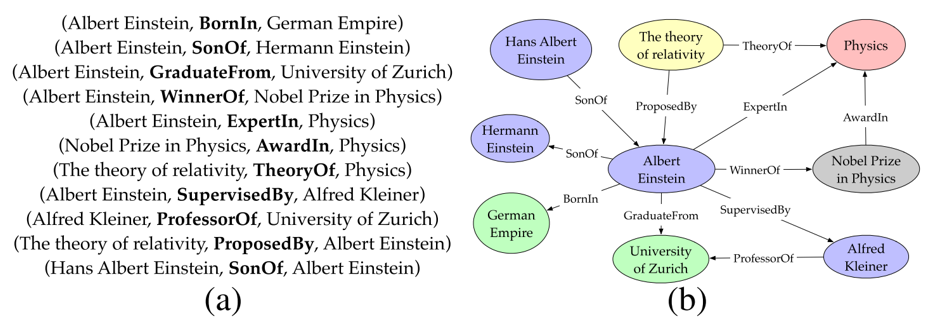
\includegraphics[width=1\textwidth]{figure/2.png}
    \caption{ An example of knowledge graph }
    \label{ Fig.2 }
\end{figure}

Due to its ability to represent a large amount of heterogeneous data, support path query, and support inference prediction tasks, Knowledge Graph has been widely used as data support in large Internet companies such as Google\cite{akerkar2009knowledge}, Alibaba\cite{li2020alimekg}, Tencent\cite{TencentKG}, and so on(Fig.\ref{ Fig.3 }), and it has also begun to be used in the field of material science to assist in material design in recent years\cite{mrdjenovich2020propnet, mccusker2020nanomine, zhao2021knowledge}. Its ability to represent a large amount of heterogeneous data can be used to represent catalytic reactions, support path query can be used to retrieve catalytic reaction paths and support inference prediction task can be used to validate the paths, allowing the automated relay catalytic path screening scheme to be implemented. In this way, different reaction information can be connected in the form of a graph by the products of the previous step reaction being the reactants of the next step reaction, and in the solution of specific problems, only the relevant knowledge applied in later decision-making on specific issues is required (Fig.\ref{ Fig.4 }).

\begin{figure}[htbp]
 \centering
 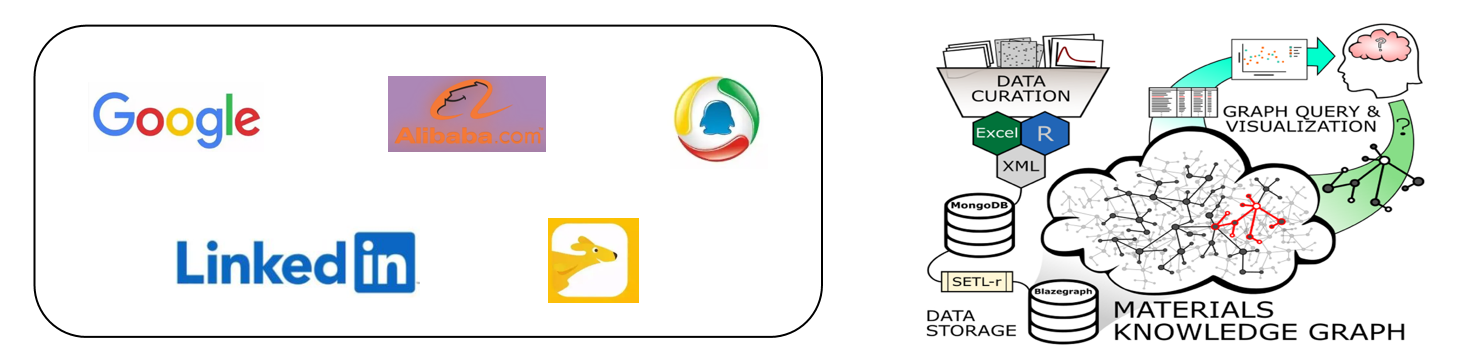
\includegraphics[width=1\textwidth]{figure/3.png}
 \caption{ Applications of Knowledge Graph }
 \label{ Fig.3 }
\end{figure}

\begin{figure}[htbp]
 \centering
 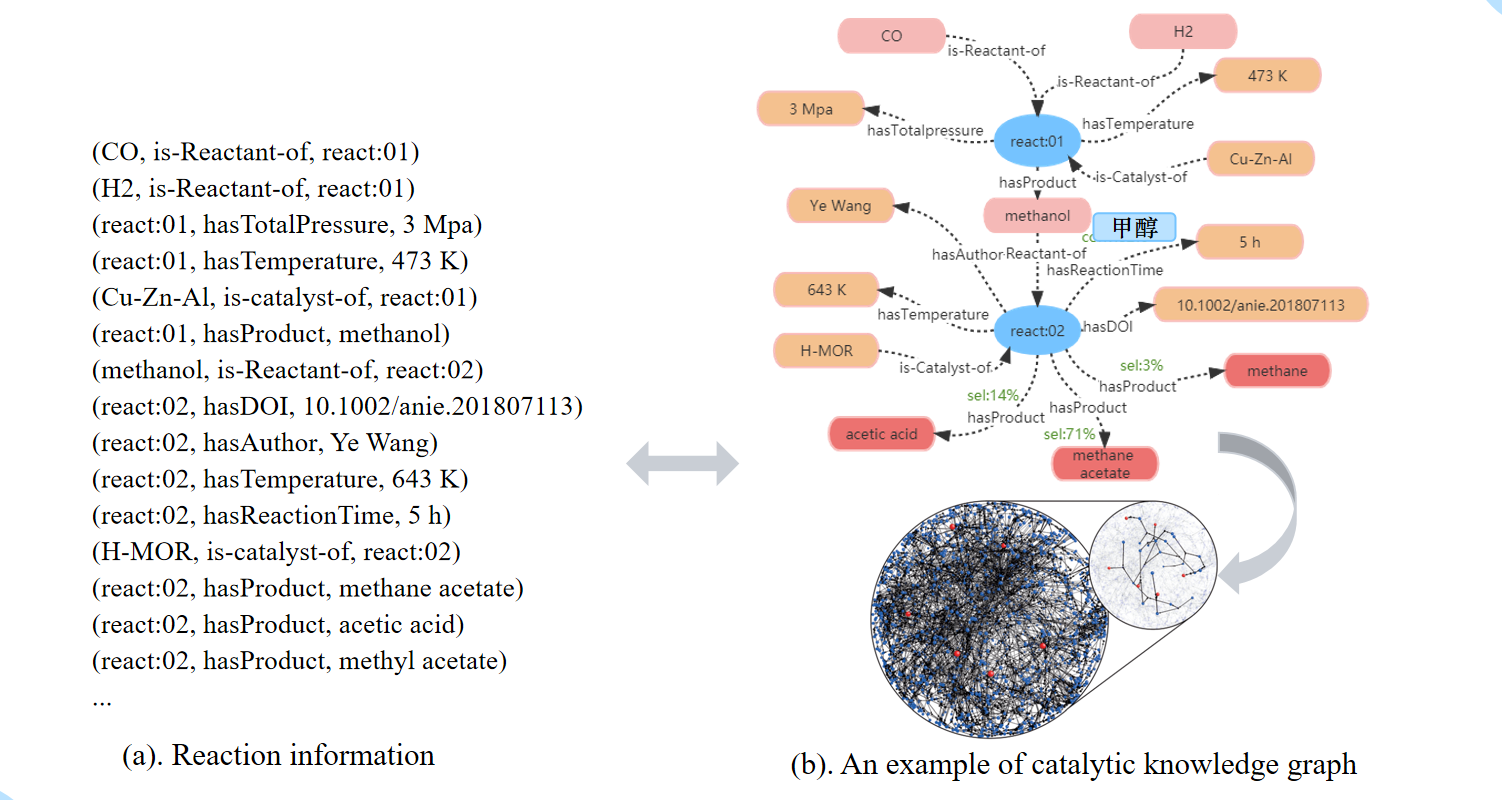
\includegraphics[width=1\textwidth]{figure/4.png}
 \caption{ Conversion between Reaction Information and Catalytic Knowledge Graph }
 \label{ Fig.4 }
\end{figure} 

\section{Related work}

\subsection{Reaction database}

Different reaction databases have been presented in recent years to handle various chemical challenges. Scifinder's web version was published in 2008\cite{gabrielson2018scifinder}, and it can be used for literature searches as well as obtaining background information on chemicals, medications, and substances. The content of SciFinder is diverse, ranging from journal papers to information on chemical structures, characteristics, and reactions.  Reaxys, a chemical information system, was introduced in 2009 to assist chemists in designing more efficient synthetic routes to molecules\cite{Reaxys}. NextMove Software released the Pistachio database in 2010\cite{pistachio}, which allows for the loading, querying, and analysis of chemical reactions. Daniel Mark Lowe created the Chemical Reaction Information Extraction System (CRIS) in 2012 to extract the USPTO reaction dataset from US patent data\cite{lowe2012extraction}. The ORD Open Source Reaction Database, a structured database that supports machine learning and associated work on reaction prediction, chemical synthesis planning, and experimental design, was published in 2021 by Conner W. Coley's group\cite{kearnes2021open}. A comparison of these databases is shown in (Table.\ref{ table.1 })

We investigated the above reaction databases and found that they all focused on the storage of organic reactions, mostly manually constructed and not easily accessible for commercial or other reasons. In addition, Pistachio and the USPTO dataset are derived from patent data without real-time effects, while SciFinder and Reaxys store reaction information in an unstructured manner. Besides, all of the above are relational databases that do not have inference capabilities. Therefore, the construction of a database for catalytic reactions became necessary.

\begin{table}[h!]
\begin{tabular}{ |p{3cm}|p{3cm}|p{3cm}|p{3cm}|p{3cm}|  }
\hline
Database&Developer&Method&Focus&Avaliability\\ \hline
CAS data(SciFinder)& ACS    &Manually curated&   Organic reactions&Not avaliable\\ \hline
Reaxys&   Elsevier  & Manually curated   &Organic reactions&For commercial use\\ \hline
Pistachio & NextMove & Java-based extraction &  Organic reactions&Not avaliable\\ \hline
AZ ELN(AstraZeneca ELN)    &AstraZeneca & Manually curated&  Organic reactions&Not avaliable\\ \hline
USPTO&   Daniel Lowe  & Java-based extraction&Organic reactions&Only <2016 avaliable\\ \hline
ORD(open reaction database) & MIT and Google  & Manually curated   &Organic or Inorganic reactions&Avaliable but manually upload\\ \hline
\end{tabular}
\caption{Existing reaction databases}
\label{ table.1 }
\end{table}

\subsubsection{Knowledge representation}

A 2012 paper published by the European Bioinformatics Institute proposed a collection of reactions from the literature for use in assisting metabolic network reconstruction as well as pathway inference\cite{alcantara2012rhea}. Rhea used CHEBI to describe the entities in the chemical reactions and the need for equilibrium in terms of the mass and charge of the reacting compounds. The reactions were manually linked to the target articles and other publicly available resources containing enzyme and pathway databases. It provides an unambiguous representation of chemical reactions:

\begin{itemize}
    \item Each of the possible reactions in  Rhea has a unique "master reaction" that is independent of any biological environment and has no associated directional information.
    \item The representation of the main reaction consists of a unique identifier, the inclusion of two reaction parts (left and right parts), a set of qualifiers describing the type of reaction and whether the reaction is balanced or not, and the current status of the reaction (approved, preliminary or obsolete), where the left and right parts of the main reaction consist of the compounds involved in the reaction, the stoichiometric coefficients.
\end{itemize}

But Rhea had some problems expressing reactions:

\begin{itemize}
    \item Inconsistent usage of generic compound names and standard nomenclature can lead to ambiguous semantic situations for reactions and compound descriptions that require manual labeling corrections
    \item Generic compound labels used to describe mixtures may introduce another ambiguity
    \item Reciprocal isomerism in the reaction introduces a third ambiguous semantic situation
\end{itemize}

To address the above issues, CHEBI identifiers, names, chemical formulae, charges, and possible 2D structures are used to define a compound in Rhea's reactions; and explicit assignments are allowed for reactions containing mixtures such as NAD+/NADH or NADP+/NADPH; and intercalation reactions for associating intercalating isomers of the same compound are provided. Although Rhea attempts to minimize or eliminate ambiguity in the description of reactions, there is some consideration for incomplete knowledge of reaction chemistry. Rhea provides incomplete reactions, where not all reactants are known and the reaction is not necessarily equilibrium. These reactions can be identified by their "preliminary" states.

Also to ensure data consistency, Rhea made the following constraints on the representation of responses:

\begin{itemize}
    \item Identical compounds (ChEBI ID, locus) could not appear on either side of the reaction. This led to the exclusion of certain common species, such as Mg2+ in Mg2+ -ATP.
    \item The mass and charge of the reaction must be chemically balanced, i.e. the compounds found in the left and right parts of the equation must have the same total number of atoms of each type and the same net charge
    \item The reaction must be unique. To ensure this uniqueness, fingerprints were calculated based on the compounds (ChEBI ID, coefficients, localization) of the two reaction parts
\end{itemize}

Each unique primary reaction in Rhea is associated with three directional reactions - forward, reverse, and bidirectional (reversible) - each with a unique identifier. However, this feature allows directional reactions from external sources to be associated with the appropriate directional reaction in Rhea. The disadvantage of this approach is that, based on current knowledge, Rhea may contain directional reactions that are not feasible in biological systems.

Each master reaction in Rhea has an administrative status, which is one of Approved, Preliminary, or Obsolete. To be approved, a reaction must satisfy the constraints described in the previous section, relating to uniqueness and equilibrium. Reactions can also have descriptive qualifiers such as "chemical equilibrium", "transport", "reaction class", and "polymerization".

\subsubsection{Reaction extraction}

There are some works about extracting reaction information from texts. Daniel Lowe downloads patent data from USPTO as an extraction source and uses machine learning and rule-based methods to extract reaction information into a representation containing atomic position information \cite{lowe2012extraction}, as shown in (Fig.\ref{ Fig.5 }), but this approach has two shortcomings, one being that the patent data does not provide a good picture of trends in the field of chemical synthesis, and the rule-based extraction of reactions results in low accuracy and low recall information.

\begin{figure}[htbp]
 \centering
 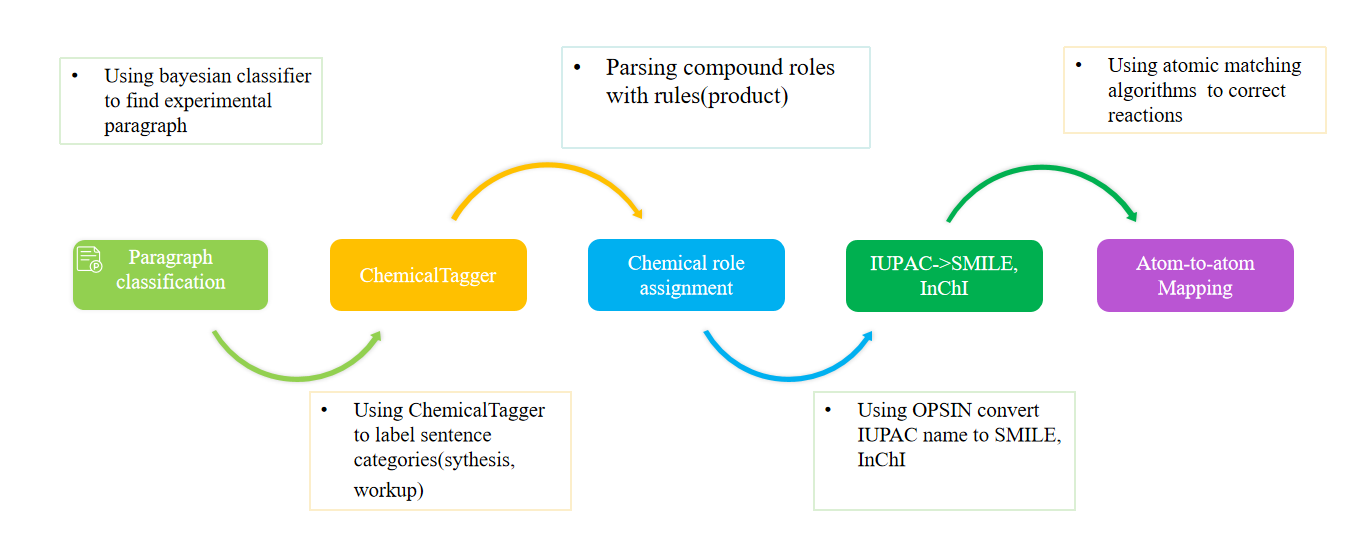
\includegraphics[width=1\textwidth]{figure/5.png}
 \caption{ Flowchart of reaction extraction from patents }
 \label{ Fig.5 }
\end{figure}

To solve these two problems, Regina Barzelay's team at the MIT Computer Science and Artificial Intelligence Laboratory published a work in 2021 that structured the reaction information into eight fields including product, reaction type, reactant, solvent, etc. With a natural language processing approach, the reaction information extraction process was divided into two parts, the entity identification task with reaction products as a central element and the relation extraction task with eight associated reaction rules, implementing the conversion of bodies of texts into structured reaction information\cite{guo2021automated}. For such work, it costs tens of students to label 9 fields of sentences from articles and spend more than 200 hours to label and check the accuracy of labeling work, which is time-consuming and labor-intensive.

To reduce the burden of manual labeling, Weiren Wang proposed a natural language processing pipeline to capture both chemical composition and property data from articles that allow analysis and prediction of superalloys. It uses a heuristic text multiple-relation extraction distance-based algorithm to get properties without any labeled samples\cite{wang2022automated}.

\subsubsection{Applications of reaction network}
Knowledge graphs have been widely used in recent years as data structures for easy storage of heterogeneous data, easy pathway retrieval and inference capabilities to aid drug discovery\cite{zeng2022toward}, disease diagnosis\cite{chai2020diagnosis} and drug detection in biomedical applications\cite{wang2021drug}, as well as in materials design to aid material selection\cite{nie2022automating}, while little has been achieved in chemistry. But recently, there have been some works about using a reaction knowledge graph to assist retrosynthesis pathway analysis\cite{jeong2022intelligent} or predict reaction outcomes\cite{nair2019data}.

Synthesis design\cite{dorwald2006side} is a formidable intellectual challenge that requires scientific intuition, experience and familiarity with a massive and rapidly growing body of knowledge and experimental data. For such a data- and knowledge-intensive paradigm, organic chemistry is notoriously deprived of computational tools that aim to assist chemists in the creative process of synthesis design. The synthetic route is a series of reactions that are started from the available molecules. The most challenging problem in the generation of synthetic routes is the large search space of the candidate reactions. 
Estimating the cost of candidate reactions has been proven effective in pruning the search space, which could achieve higher accuracy with the same search iteration.

% “Found in Translation”: predicting outcomes of complex organic chemistry reactions using neural sequence-to-sequence models
Multiple efforts have been made in the past 50 years to rationalize a large number of chemical compounds and reactions identified, which forms the large knowledge bases for solving synthetic problems. In 1969, Corey and Wipke\cite{corey1969computer} demonstrated that both synthesis and retrosynthesis could be performed by a machine. Their pioneering contribution involved the use of handcrafted rules made by experts, which are commonly known as reaction templates. The templates encode the local changes to the atoms' connectivity under certain conditions accounting for various subtleties of retro-synthesis. A similar algorithm emerged in the late 1970s\cite{salatin1980computer} which also requires a set of expert rules. Unfortunately, rules writing is a tedious task, both time and labor-intensive, and may not cover the entire domain for complex organic chemistry problems. In such cases, profound chemical expertise is still required, and the solutions are usually developed by trained organic chemists.
However, it can be extremely challenging even for them to synthesize a relatively complex molecule, which may take several reaction steps to construct. Navigating the chemical space of drug-related compounds by relying only on Intuition may turn a synthesis into a nearly impossible task, especially if the problem is slightly outside the expert's knowledge. Other approaches extract reaction templates directly from data. In this specific context, candidate products are generated from the templates and then ranked according to their likelihood. Satoh and Funatsu\cite{satoh1995sophia, satoh1996further} used various hard-coded criteria to perform the ranking whereas more recent approaches\cite{segler2017neural,struble2020current} used a deep neural network. However, these types of approaches are fundamentally dependent on the rule-based system component and thus inherit some of its major limitations. In particular, these approaches do not produce sufficiently accurate predictions outside of the training domain.

% A chemically consistent graph architecture for massive reaction networks applied to solid electrolyte interphase formation
The first-ever electrochemical reaction network is constructed from the first principles of thermodynamic calculations to describe the formation of the Li-ion solid electrolyte interphase (SEI), which is critical for the passivation of the negative electrode. Optimized shortest path algorithms like Dijkstra's and Yen's are allowed to be used to identify the best or N-best reaction paths to any given molecule node in any chemical reaction network for the first time. This network comprises nearly 6000 species and 4.5 million reactions\cite{blau2021chemically}.
% Parallel Optimization of Synthetic Pathways within the Network of Organic Chemistry
While it is simply beyond the cognition of any individual human to understand and analyze all this collective chemical knowledge, modern computers have become powerful enough to perform suitable network analyses within reasonable timescales. Therefore, Kowalik first represents a reaction network with a bipartite graph and uses a recursive algorithm that back-propagates on the network starting from a specified target molecule to examine possible syntheses. Then, a cost calculation continues recursively, moving backward from a target until a critical search depth is reached. This algorithm rapidly identifies the synthetic plan which minimizes the cost criterion\cite{kowalik2012parallel}.
% Data-driven computer-aided synthesis design
Reaction prediction is closely related to the problem of synthetic route prediction. 
Leveraging reaction prediction capabilities toward full synthesis design poses various challenges. 
Primarily it requires advanced strategic reasoning algorithms to mitigate the combinatorial explosion, 
and it requires filtering out invalid suggestions to guarantee the chemical integrity of solutions\cite{ravitz2013data}.
% prediction-of-compound-synthesis-accessibility-based-on-reaction-knowledge-graph
With the increasing application of deep learning-based generative models for de novo molecule design, quantitative estimation of molecular synthetic accessibility becomes a crucial factor for prioritizing the structures generated from generative models. On the other hand, it is also useful for helping prioritization of hit/lead compounds and guiding retro-synthesis analysis. Based on the USPTO and Pistachio reaction datasets, Baiqing Li created a refined chemical reaction network, in which a depth-first search was performed to identify the reaction paths of product compounds. This reaction dataset was then used to build a predictive model for distinguishing the organic 
compounds either as synthesize (ES) or hard-to-synthesize (HS) classes. Three synthesis accessibility (SA) models were built using deep learning/machine learning algorithms\cite{li2022prediction}.
% GNN-Retro: Retrosynthetic Planning with Graph Neural Networks
To get a better performance in reaction prediction, a new framework is proposed, named GNN-Retro, for retrosynthetic planning problems by combining graph neural networks (GNN) and the latest search algorithm. 
The structure of GNN in this framework could incorporate the information of neighboring molecules, which will improve the estimation accuracy of this framework\cite{han2022gnn}.
% “Found in Translation”: predicting outcomes of complex organic chemistry reactions using neural sequence-to-sequence models
Schwaller cast the reaction prediction task as a translation problem by introducing a template-free sequence-to-sequence model, trained end-to-end and fully data-driven. A tokenization is proposed, which is arbitrarily extensible with reaction information\cite{schwaller2018found}.
% Modelling Chemical Reasoning to Predict Reactions
Knowledge graph-based inferential prediction capabilities enable the search for organic synthesis and new conversions, and predicting reactants' reactivity is crucial for predicting reactions\cite{coley2019graph}. However, the prediction of reactivity is limited by a set of conditions, including reactants, and catalysts, and therefore, reaction prediction at a broad level includes the prediction of products, catalysts, and reagents under the conditions of a given reactant. Expert systems, which extract reaction rules based on manual input or algorithms, are the most widely used method for predicting reactions\cite{chen2009no, gasteiger1987new, marcou2015expert, patel2020savi}. However, this approach has several drawbacks: 1. They require the expert to encode knowledge manually rather than using it directly as reaction rules or extracting rules from data using heuristics; 2. It is very difficult to maintain such a system, and 3. These rules do not generalize. Expert systems can only use existing rules to predict reactions encoded with these rules and cannot discover new chemical information. To address this problem, in 2017 Mark P. Waller published a paper introducing a new approach to predicting reactions, assuming that to predict a reaction that has not been seen before, ignoring its reaction type, one must find the missing link of the reactant molecule in the currently collected knowledge graph\cite{segler2017modelling}. The paper views the problem of predicting the outcome of a reaction as a link prediction problem in a knowledge graph and uses the concept of half-reactions, where a binary reaction can be split into two half-reactions, with one half-reaction containing how the atoms and bonds of the reactants are converted and merged in the product. By relying on combining the results of the two half-reactions, the final product can be obtained. At the same time, an initial reaction condition is obtained by combining the conditions of the first reaction and the last reaction to obtain an initial reaction condition that is predicted for that reaction. This method does not pay much attention to catalyst, reaction type, reaction mechanism, and reactivity, but only focuses on the reaction diagram itself to get the possible products, and the reaction conditions can be solved by a simple union, as shown in (Fig.\ref{ Fig.6 }).

\begin{figure}[htbp]
 \centering
 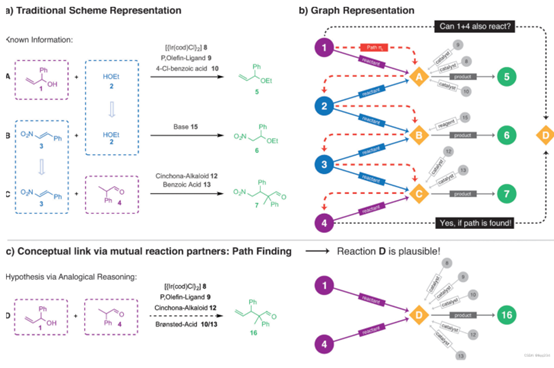
\includegraphics[width=0.7\textwidth]{figure/6.png}
 \caption{ A scheme representation (a) can be translated into a graph representation (b). Numbered nodes correspond to molecules (circles); reaction nodes(diamonds) are designated with a letter. The graph representation allows a fine-grained encoding of the roles molecules can play in a reaction and can be used to study the relationships of molecules. cod = 1,5-cyclooctadiene. c) To predict the reaction of 1 and 4, we perform a path search and retrieve path 1!A!2!B!3!C!4 (red dotted line). This corresponds to a logical explanation: because 1 and 3 react with 2, they have analogous reactivity, and 3 and 4 have complementary reactivity, compounds 1 and 4 are likely also to react. From the retrieved path, we can predict the possible product and the needed catalysts and reagents by concatenation of half-reactions (see the left-hand side). }
 \label{ Fig.6 }
\end{figure}

\subsection{Knowledge graph construction}

In May 2012, the foreign search engine company Google for the first time proposed a Knowledge Graph\cite{fensel2020introduction}, prompting great concern in academia and industry, The domestic search engine company Baidu and Sogou have also constructed their knowledge graph\cite{yu2017knowledge, SogouKG}. Along with the emergence of Knowledge Graph, the search engine from the original string-matching query into a semantic search\cite{zhu2017intelligent}, greatly improving the quality of the original search. The construction of a high-quality and complete knowledge graph, not only in the semantic search, automatic question and answer system\cite{he2021optimizing, abujabal2017automated, saha2018complex}, artificial intelligence and other research directions has a high research value, but also in the medical, commercial, financial and other fields have a wide range of applications\cite{li2020real, elhammadi2020high}. In recent years, knowledge graphs have also been used to assist material design in the field of material science. The building of knowledge graphs is a critical step in achieving the use of knowledge graphs in the field of catalysis, such as the relay catalysis automatic path screening system described in this study.

The architecture of the knowledge graph, including the logical structure of the knowledge graph itself and the technical (system) architecture used to construct the knowledge graph\cite{hao2021construction}. The knowledge graph can be logically divided into 2 levels: the data layer and the schema layer, as shown in (Fig.\ref{ Fig.7 }). In the data layer of the knowledge graph, knowledge is stored in the graph database in units of facts. For example, Virtuoso\cite{Virtuoso} and Jena\cite{Jena} are typical graph databases. If "entity-relationship-entity" or "entity-attribute-attribute-value" triples are used as the basic expression of facts, all the data stored in graph databases will constitute a huge entity-relationship network, forming a knowledge "graph". 

The schema layer is above the data layer and is the core of the knowledge graph. What is stored in the schema layer is refined knowledge, and ontology libraries are usually used to manage the schema layer of the knowledge graph, with the help of the ontology library's ability to support axioms\cite{krotzsch2017ontologies}, rules and constraints to standardize the links between entities, relationships and objects such as entity types and attributes. The position of ontology libraries in knowledge graphs is equivalent to the mold of knowledge bases, and knowledge bases with ontology libraries have less redundant knowledge.

\begin{figure}[htbp]
 \centering
 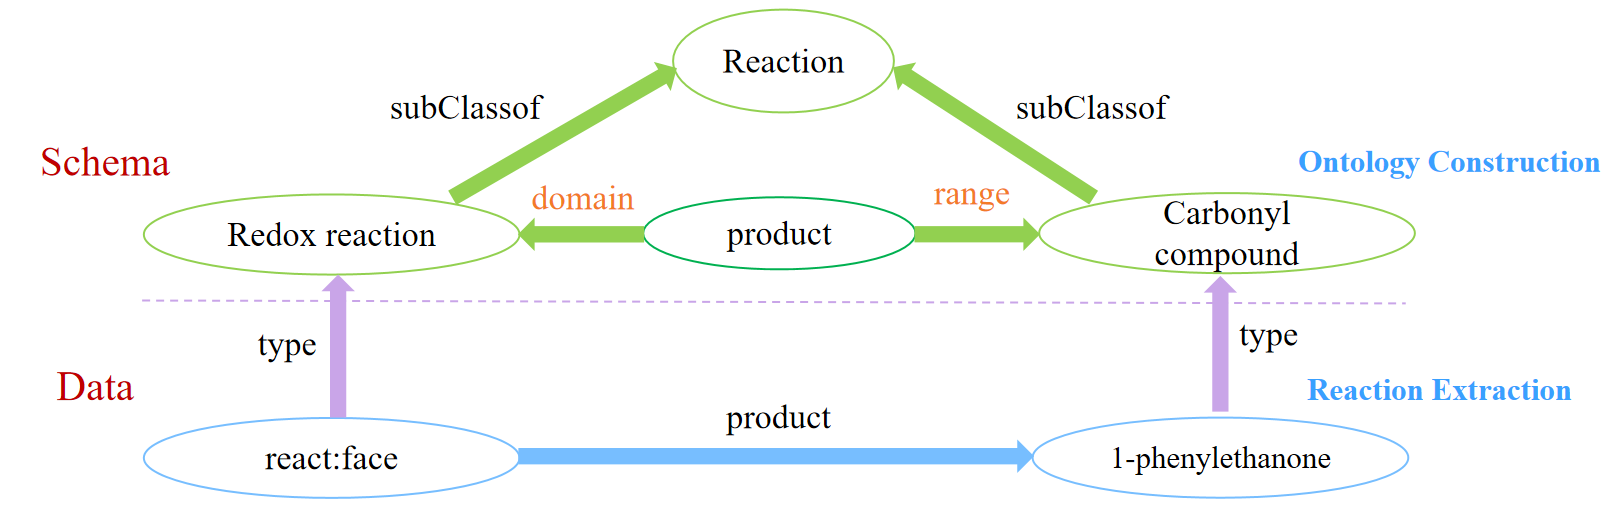
\includegraphics[width=1\textwidth]{figure/7.png}
 \caption{ Schema layer and data layer of a knowledge graph }
 \label{ Fig.7 }
\end{figure}

The process of building a knowledge graph starts from the raw data and uses a series of automated or semi-automated technical means to extract knowledge elements (facts) from the raw data and store them in the data and schema layers of the knowledge base\cite{gutierrez2021knowledge}. It is an iterative updating process and according to the logic of knowledge acquisition\cite{dai2019distantly}, each iteration consists of three stages: information extraction, knowledge fusion and knowledge processing, as shown in(Fig.\ref{ Fig.8 }). 

The initial step in knowledge graph building is information extraction\cite{muhammad2020open}, where the key issue is how to automatically extract information from heterogeneous data to obtain candidate knowledge units. Information extraction is a technique for automatically extracting structured information from semi-structured and unstructured data, such as entities, relationships, and entity properties. Entity extraction, relationship extraction, and attribute extraction are the major approaches involved.

\begin{figure}[htbp]
    \centering
    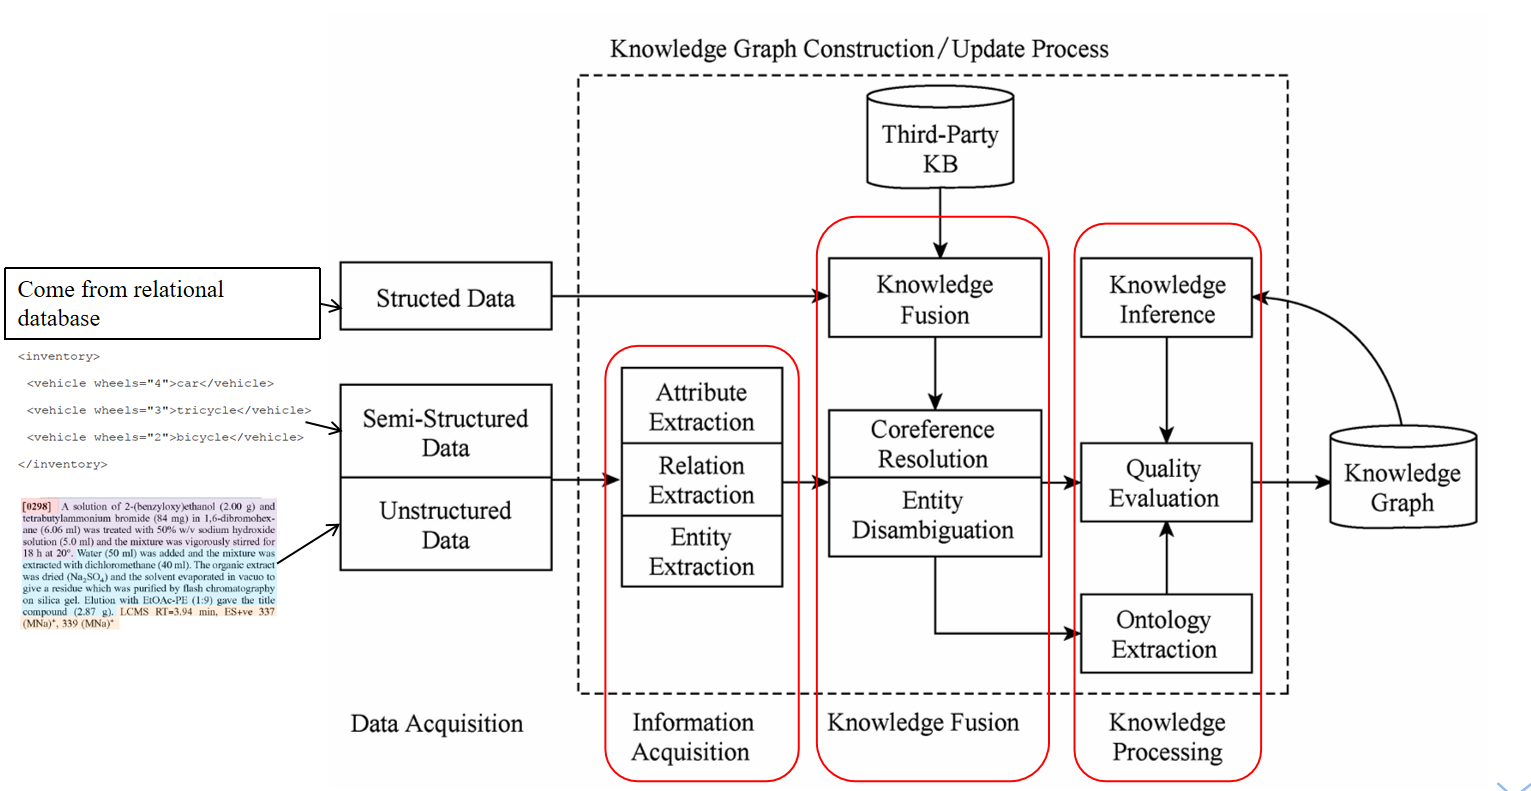
\includegraphics[width=1\textwidth]{figure/8.png}
    \caption{ Construction of a knowledge graph }
    \label{ Fig.8 }
\end{figure}

\subsubsection{Entity recognition}
Entity recognition refers to recognizing named entities from text and classifying them into predefined classes\cite{al2020named}.
In general, existing methods can be divided into the rule-based method, statistical model-based approach and 
deep learning-based approach.
% Rule-based approach
The rule-based approach is the early method of writing hand-curated rules, such as regular matching, curated by specialists in a specific domain. This extraction style can achieve high accuracy and recall when it is used on small datasets. However, as the dataset grows, the rule-set construction cycle becomes longer and less flexible\cite{alfred2014malay}.
% Statistical model-based approach
The statistical model-based approach trains the model with a completely annotated corpus or partially annotated corpus.
The main models used are Hidden Markov Model \cite{fine1998hierarchical}, Conditional Markov Model \cite{cook2004conditional}, 
Maximum Entropy Model \cite{ratnaparkhi1996maximum} and Conditional Random Fields Model\cite{wallach2004conditional}. 
These methods regard entity recognition as a sequence-to-sequence problem. Compared to the general classification task, the prediction of the current label for the sequence labeling task is not only relevant to the current input but also to previously predicted labels.  
% Deep learning-based approachwang2020recent
With the widespread adoption of deep learning methods in the field of natural language processing, the deep neural network is applied to entity recognition with good effects. In contrast to traditional statistical models, deep learning-based approaches take a vector of words in the text as input directly and implement end-to-end named entity recognition through neural networks, no longer relying on manually defined features.
Currently, major neural networks used for named entity
recognition is Convolutional Neural networks (CNN)\cite{o2015introduction}, Recurrent Neural networks (RNN) \cite{medsker2001recurrent} and neural networks that introduces the Attention Mechanism\cite{tilk2016bidirectional}. In general, the different Neural network structures act as encoders in the named entity recognition process, obtaining a new vector representation of each word based on the initial input and the contextual information of the word, and finally outputting the annotation results for each word through a CRF model.
% Chemical entity recognition
The emergence of "big data" initiatives has led to the need for tools that can automatically extract valuable information from large volumes of unstructured data, such as the scientific literature. Since chemical information can be present in figures, tables, and textual paragraphs, successful information extraction often depends on the ability to interpret all of these domains simultaneously. A complete toolkit is present for the automated extraction of chemical entities and their associated properties, measurements, and relationships from scientific documents that can be used to populate structure chemical databases\cite{swain2016chemdataextractor}. It uses unsupervised word clustering based on a massive corpus of chemistry articles to achieve chemical-named entity recognition with an F-score of 93.4$\%$.

\subsubsection{Relation extraction}
Relation extraction is one of the most important sub-tasks of knowledge extraction for unstructured text data, where the semantic relationship between two or more entities is extracted from the text. Relation extraction is closely related to entity extraction, generally after identifying the entities in the text, then extracting the possible relationships between them, or many joint models do both tasks together\cite{yu2020relationship}. The following are some of the main methods for extracting relations.

\paragraph{Templete-based approach}
For the text "water is a reactant of WGS reaction", the pattern can be constructed as "[1] is a reactant of [2]". We can get entities for "is a reactant of" relation with this pattern. The advantage of the template-based relationship extraction approach is that templates are simple to construct and allow relatively quick implementation of relationship extraction systems on small datasets. Similarly, when the data size is large, manual construction of templates takes a lot of time for domain experts. In addition, template-based relationship extraction systems are less portable, requiring the templates to be rebuilt when faced with the same problem in another domain. Finally, the recall rate of template-based relationship extraction systems is generally low due to the limited number of manually constructed templates and the insufficient coverage of templates\cite{flynn2007automated, romano2006investigating}.

\paragraph{Supervised learning-based approach}
Supervised learning-based relationship extraction methods transform relationship extraction into a classification problem by training a supervised learning model for relationship extraction based on a large amount of annotated data\cite{onishi2018relation, timoshenko2017supervised, ciaburro2021machine}. The general steps in relationship extraction using supervised learning methods include: predefining the type of relationship; manually annotating the data; and designing the features required for relationship recognition (relying on feature engineering\cite{turner1999conceptual}), which are typically computed based on the context of the sentence in which the entity is located; selecting a classification model (e.g. support vector machines\cite{huang2018applications}, neural networks and naive Bayes \cite{frasconi2001text}) and training the model based on the annotated data; and evaluating the trained model.

\paragraph{Deep learning-based approach}
At present, existing deep learning-based relation extraction methods can be divided into two classes: pipelined method and joint extraction method\cite{zheng2017joint}.
The pipeline method treats entity recognition and relation extraction as two separate processes that 
do not affect each other, but the relation extraction task is performed based on the results of entity recognition,
Therefore, the results of relation extraction rely on that of entity extraction such as CR-CNN\cite{nogueira2015classifying},
Att-Pooling-CNNs\cite{li2018attention} and Att-BLSTM\cite{chen2018wifi}. These methods have the following disadvantages:
\begin{itemize}
    \item[1] Error propagation, where errors in the entity recognition module affect the performance of the following relation extraction.
    \item[2] Ignoring the relation between the two subtasks.
    \item[3] Unnecessary redundant information is generated as the identified entities are paired in pairs and then classified relationally, those unrelated entity pairs introduce redundant information and raise the error rate.
\end{itemize}
Joint extraction methods combine entity extraction and relation extraction, where a sentence is an input and a triplet of entities with relations is directly obtained by a joint model of entity recognition and relation extraction. This can overcome the drawbacks of the pipelined approach above, but probably cause more 
complex structures such as BERT \cite{tenney2019bert}, LSTM-RNN \cite{selvin2017stock}, DGCNN \cite{phan2018dgcnn}, etc.

\paragraph{Weakly supervised learning-based approach}
Supervised learning-based relationship extraction methods require a large training corpus, especially for deep learning-based methods, where the optimization of the model relies more on a large amount of training data. When the training corpus is insufficient, weakly supervised learning methods can use only a small amount of annotated data for model learning. Weakly supervised learning-based relationship extraction methods mainly include remotely supervised methods and Bootstrapping methods.

% remotely supervised methods
The remotely supervised approach automatically constructs a large amount of training data by aligning the knowledge graph with unstructured text, reducing the model's reliance on manually 
annotated data and enhancing the model's cross-domain adaptability. The underlying assumption of the remotely supervised approach is that if two entities have some relationship in the knowledge graph, then the sentences containing both entities express that relationship. The remotely supervised relation extraction method can make use of the rich knowledge graph information to obtain training data, effectively reducing the workload of manual annotation. However, based on the assumption of remote supervision, a large amount of noise will be introduced into the training data, thus triggering the phenomenon of semantic drift. Existing work includes PCNNs (Piecewise Convolutional Neural Networks) \cite{ji2008mixed} and CNN-RL\cite{wen2020new}.

% Bootstrapping methods
The Bootstrapping method originates from the autonomous sampling method in statistics, 
which uses a small number of instances as an initial seed set, then learns on the seed set 
to obtain a template for relationship extraction, and then uses the template to extract more instances to be added to the seed set. Through continuous iteration, the Bootstrapping method can extract a large number of instances of a relationship from the text. Several entity relationship extraction systems use the Bootstrapping approach, such as DIPER \cite{gallet2015diuretic}, Snowball \cite{agichtein2000snowball} and NELL, but they are out-update. 
The advantages of the Bootstrapping approach are that the relationship extraction system is cheap to build, suitable for large-scale relationship extraction tasks, and can discover new relationships. 
However, the sensitivity to initial seeds, the problem of semantic drift and the low accuracy of the results have made the bootstrapping method fade out of the limelight.

\subsubsection{Ontology construction}
Ontologies are used to define concepts in a particular domain and the relationships between concepts, which is the schema layer of a knowledge graph. They serve two purposes: to constrain the data and to facilitate knowledge graph queries. Since the various compounds in chemistry are more clearly defined and related to each other.
Ontologies can be built in a top-down seven-step process(Fig.\ref{ Fig.9 }), which is simply divided into reusing existing ontologies and building custom ontologies using build tools\cite{subhashini2011survey}.

\begin{figure}[htbp]
 \centering
 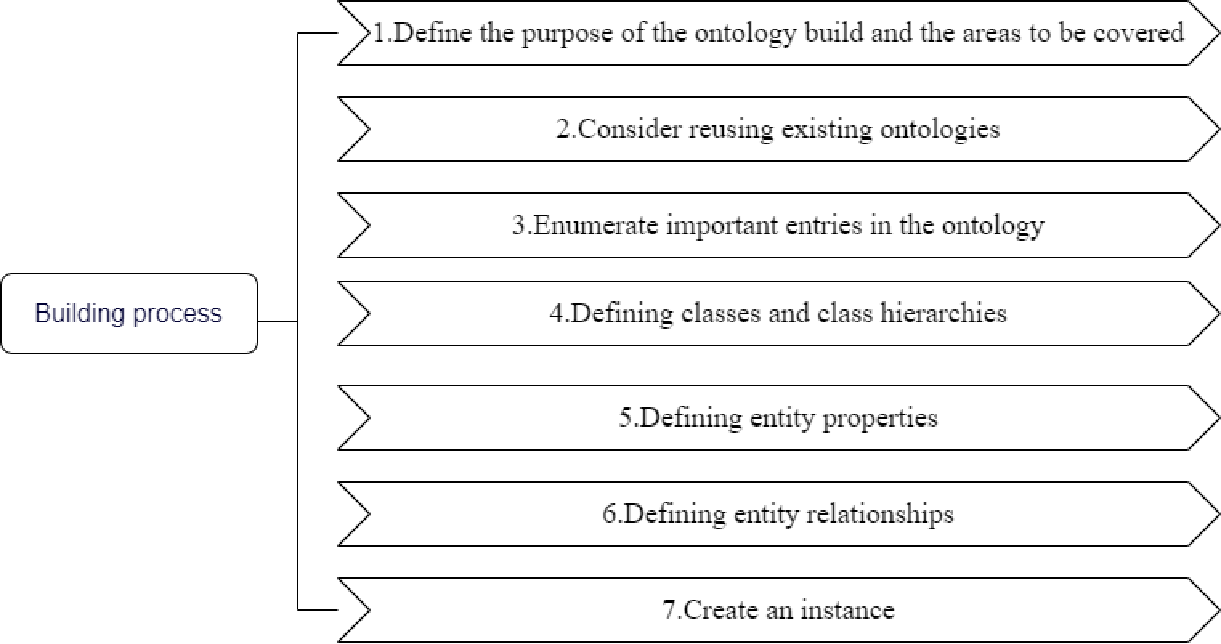
\includegraphics[width=0.7\textwidth]{figure/9.png}
 \caption{ A top-down seven-step process of building an ontology }
 \label{ Fig.9 }
\end{figure}

The development of chemical ontologies is in the beginning. There are very few ontologies to be found for this specific field. ChEBI\cite{degtyarenko2007chebi} is a database of compounds published in 2007 that describes small molecule compounds in biochemistry using standard bioinformatics terminology, providing compound names, structures, descriptors and ontology information. Here is the ontological structure of cobalt in CHEBI and the relationship between a cobalt atom (Fig.\ref{ Fig.10 }), 
and a metal atom. Due to its organic and inorganic content and clear structure, the ZOOMA tool (Fig.\ref{ Fig.11 }) provides the possibility of converting chemical names in the text into ontology corresponding categories to be used as the basic ontology of the catalytic knowledge base about specific data. For categories that cannot be represented by the basic ontology, the semi-automated ontology building tool Protege\cite{musen2015protege} can be used to build the relevant concepts and relationships on its own, thus completing the construction of the schema layer.

Name reactions serve a key purpose in chemistry as they provide a certain keyword for a given reaction, its reactants and products as well as data about the reaction environment. The RXNO\cite{pachl2020overview} is by far the most complete ontology about name reactions. It contains over 500 name reactions, sorted into an ontology with several layers, as shown in (Fig.\ref{ Fig.12 }). In the first instance, the reactions are sorted by the general type of the reaction, e.g.oxidations or cyclizations. The second layer divides the reactions further into smaller categories, for example, their dedicated reactants. Again, using the example of oxidations, they are further divided into reactions describing the synthesis of alcohols or alkenes. Using this tree structure, a reaction can be obtained that is explicitly designed for a given goal. However, despite the enormous amount of reactions, sorted into this system, there is no further information given about these, aside from their name and parents. Also, certain chemicals, that are needed for the reaction, are assigned to the process and vice versa.


\begin{figure}[htbp]
 \centering
 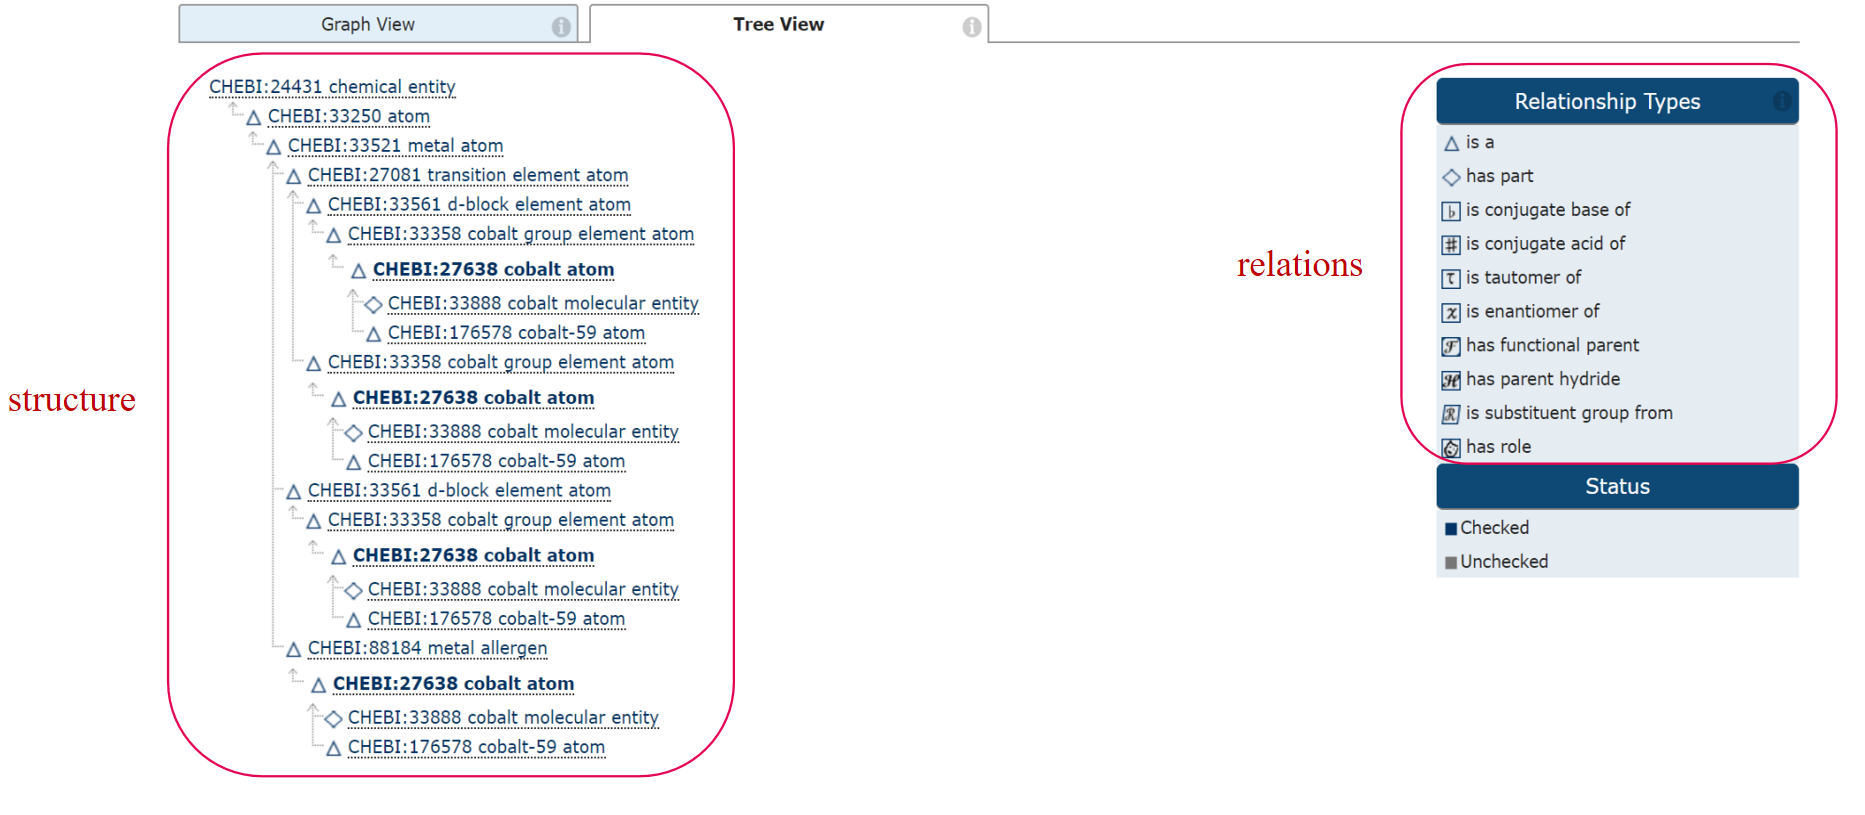
\includegraphics[width=0.7\textwidth]{figure/10.png}
 \caption{ Ontology structure of Co }
 \label{ Fig.10 }
\end{figure}

\begin{figure}[htbp]
 \centering
 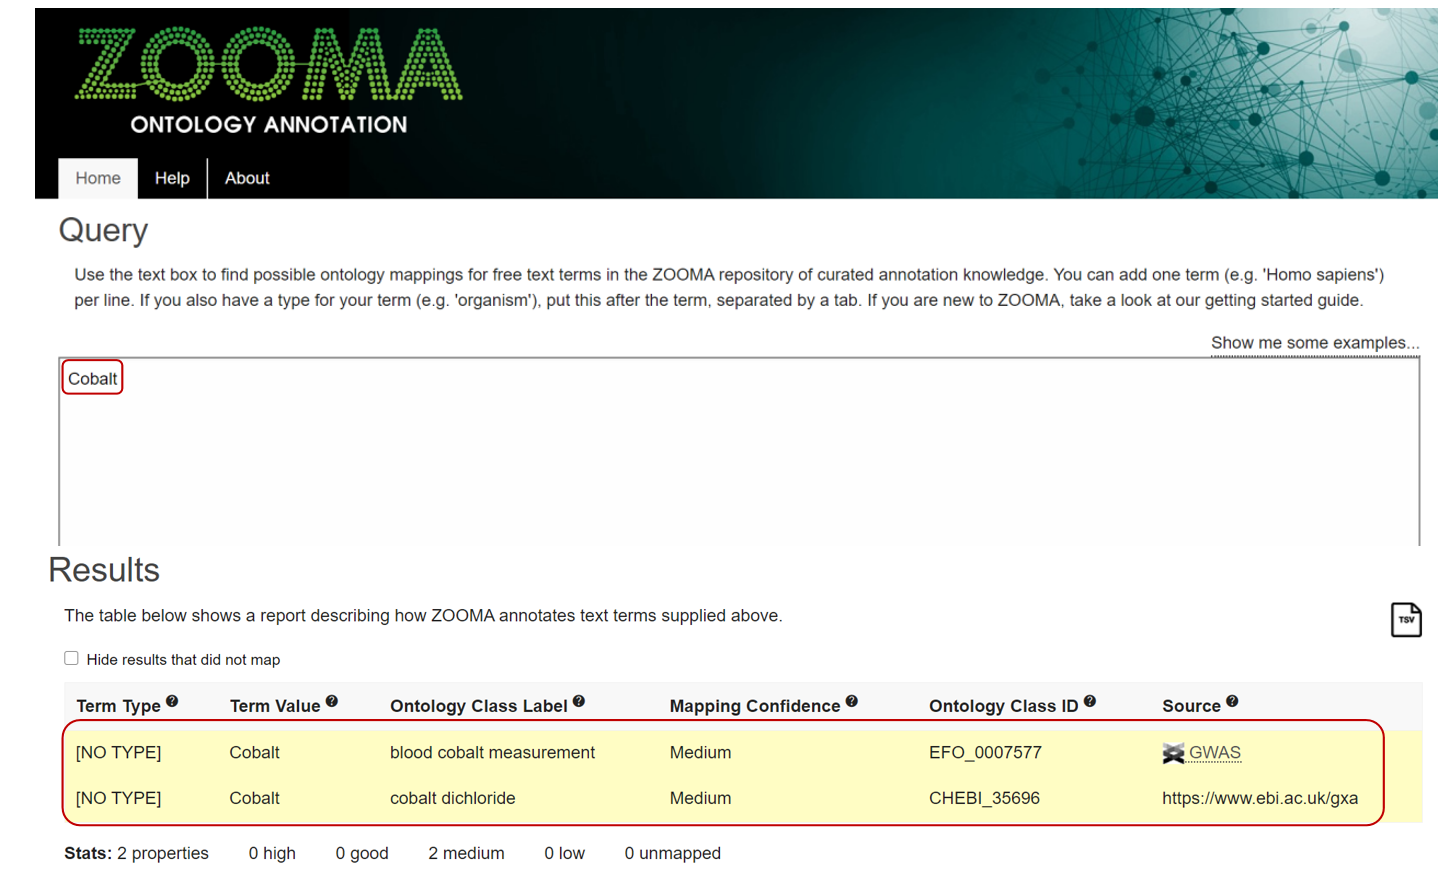
\includegraphics[width=0.7\textwidth]{figure/11.png}
 \caption{ An example of ZOOMA search }
 \label{ Fig.11 }
\end{figure}

\begin{figure}[htbp]
 \centering
 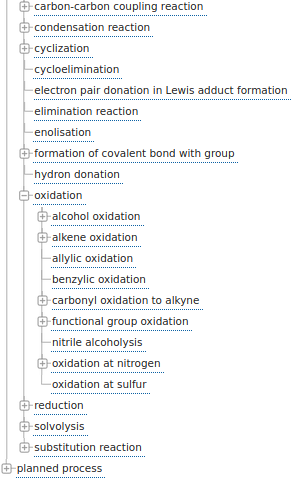
\includegraphics[width=0.7\textwidth]{figure/12.png}
 \caption{ Exemplary branch of the RXNO (derived by [44])}
 \label{ Fig.12 }
\end{figure}

\section{Research Methods and Progress}

To build the catalytic knowledge graph, we divided the work into 4 parts: Schema design, Article collection, Reaction extraction and Knowledge graph construction.

\subsection{Schema design}
To construct a knowledge graph that can be used in the study of catalytic reactions, we need to explicitly represent a catalytic reaction, and here we have designed preliminary data layers.
Firstly a reaction consists of reactants, products, catalysts, solvents, intermediates, products and reaction conditions.
For the structure of the whole reaction, we would like a reaction to be represented as a graph structure as shown in (Fig.\ref{ Fig.13 }).
\begin{figure}[htbp]
 \centering
 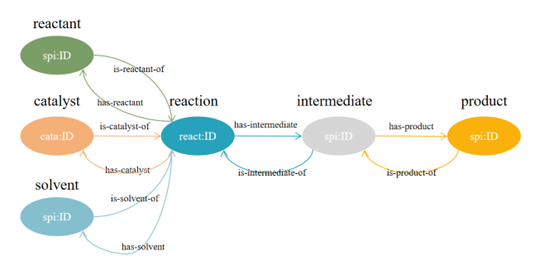
\includegraphics[width=0.7\textwidth]{figure/13.png}
 \caption{ Schematic of a Catalytic Knowledge Graph }
 \label{ Fig.13 }
\end{figure}

Where reactant, catalyst, solvent, reaction, intermediate, and product represent the node type of a catalytic reaction in the knowledge graph.

For the above nodes, they contain the following attributes as shown in (Fig.\ref{ Fig.14 }).

\begin{figure}[htbp]
 \centering
 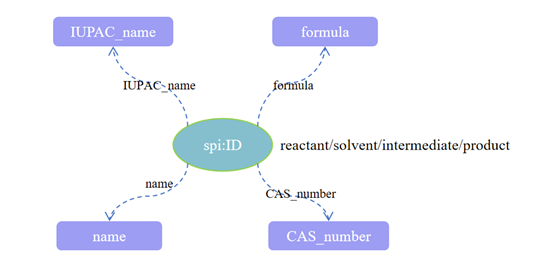
\includegraphics[width=1\textwidth]{figure/14.png}
 \caption{ The structure of Reactant/Solvent/Intermediate/Product }
 \label{ Fig.14 }
\end{figure}

Also, the reacting node contains information such as reaction conditions, as shown in (Fig.\ref{ Fig.15 }).
\begin{figure}[htbp]
 \centering
 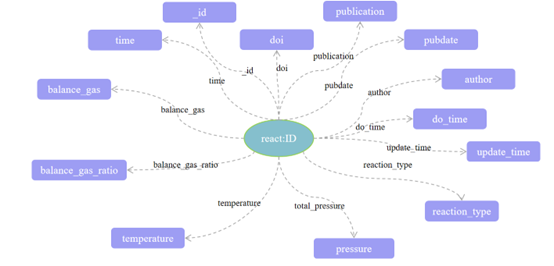
\includegraphics[width=1\textwidth]{figure/15.png}
 \caption{ The structure of reaction node in catalytic knowledge graph }
 \label{ Fig.15 }
\end{figure}

The structure of the catalyst node is shown in (Fig.\ref{ Fig.16 }).

\begin{figure}[htbp]
 \centering
 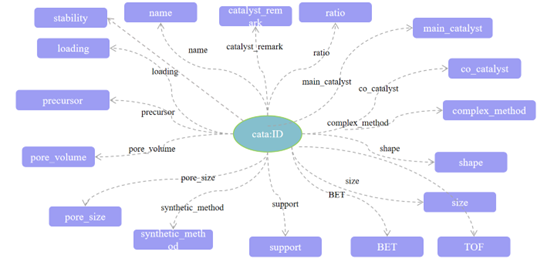
\includegraphics[width=1\textwidth]{figure/16.png}
 \caption{ The structure of catalyst node in catalytic knowledge graph }
 \label{ Fig.16 }
\end{figure}

\subsection{Article collection}
To obtain the reaction data, we grabbed data from 12303 papers from ACS, Elsevier, Nature, and Science using the keywords heterogeneous catalysis, syngas, and catalytic hydrogenation reaction using the selenium tool, the literature collection result as shown in (Fig.\ref{ Fig.17 }).

\begin{figure}[htbp]
 \centering
 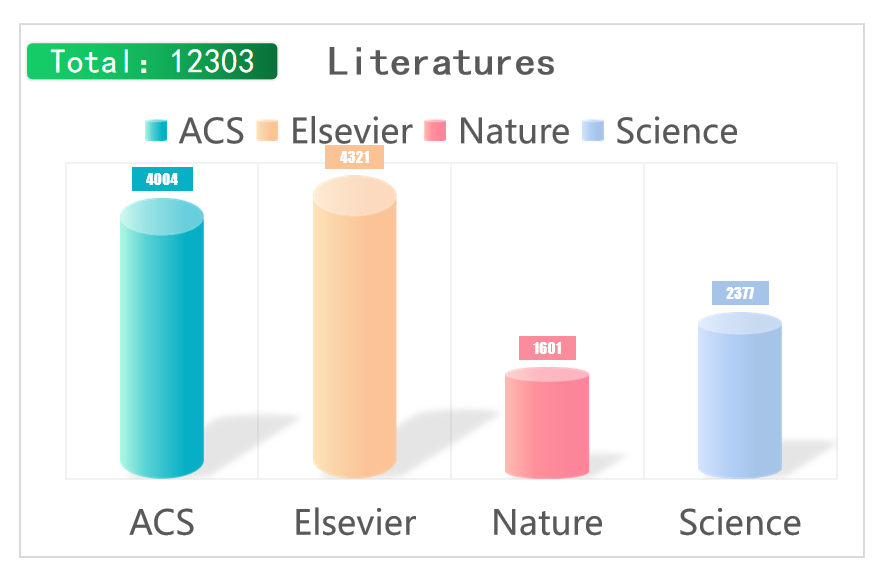
\includegraphics[width=1\textwidth]{figure/17.png}
 \caption{ Literatures }
 \label{ Fig.17 }
\end{figure}



\subsection{Reaction extraction}

\paragraph{Reaction information extraction}To extract reactions from articles, we try to divide the extraction task into two parts-reaction extraction from text, and reaction extraction from tables. To achieve reaction extraction from text, we first need to know if the current paragraph contains the target reaction information or not. We use "selectivity" and "\%" as keywords to determine whether a paragraph contains reactive information.
% 尝试规则提取化合物与属性
If the current paragraph contains the target reaction information, we use chatgpt's interface to design the prompt to get the response information in it, as shown in (Fig.\ref{ Fig.18 }). 
\begin{figure}[htbp]
 \centering
 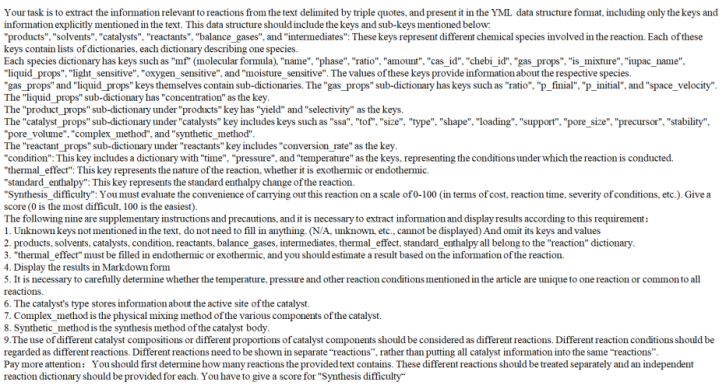
\includegraphics[width=0.7\textwidth]{figure/18.png}
 \caption{ Example of Prompt }
 \label{ Fig.18 }
\end{figure}

For table data, we use a rule-based approach to get relevant reaction information. Finally, the text and table responses are fused together to form a more complete response message.

\paragraph{Data validation}In order to ensure the accuracy and completeness of the data, we also need to carry out data validation of the extracted information to ensure the accuracy of the data by manual calibration as shown in (Fig.\ref{ Fig.19 }).

\begin{figure}[htbp]
 \centering
 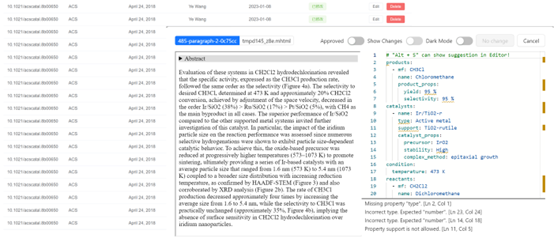
\includegraphics[width=0.7\textwidth]{figure/19.png}
 \caption{ Validation of extracted reaction information }
 \label{ Fig.19 }
\end{figure}

\subsection{Catalytic knowledge graph construction and applications}

\paragraph{RDF data conversion}For the data after validation, we need to convert it into RDF form to store it in the graph database, as shown in (Fig.\ref{ Fig.20 }).

\begin{figure}[htbp]
 \centering
 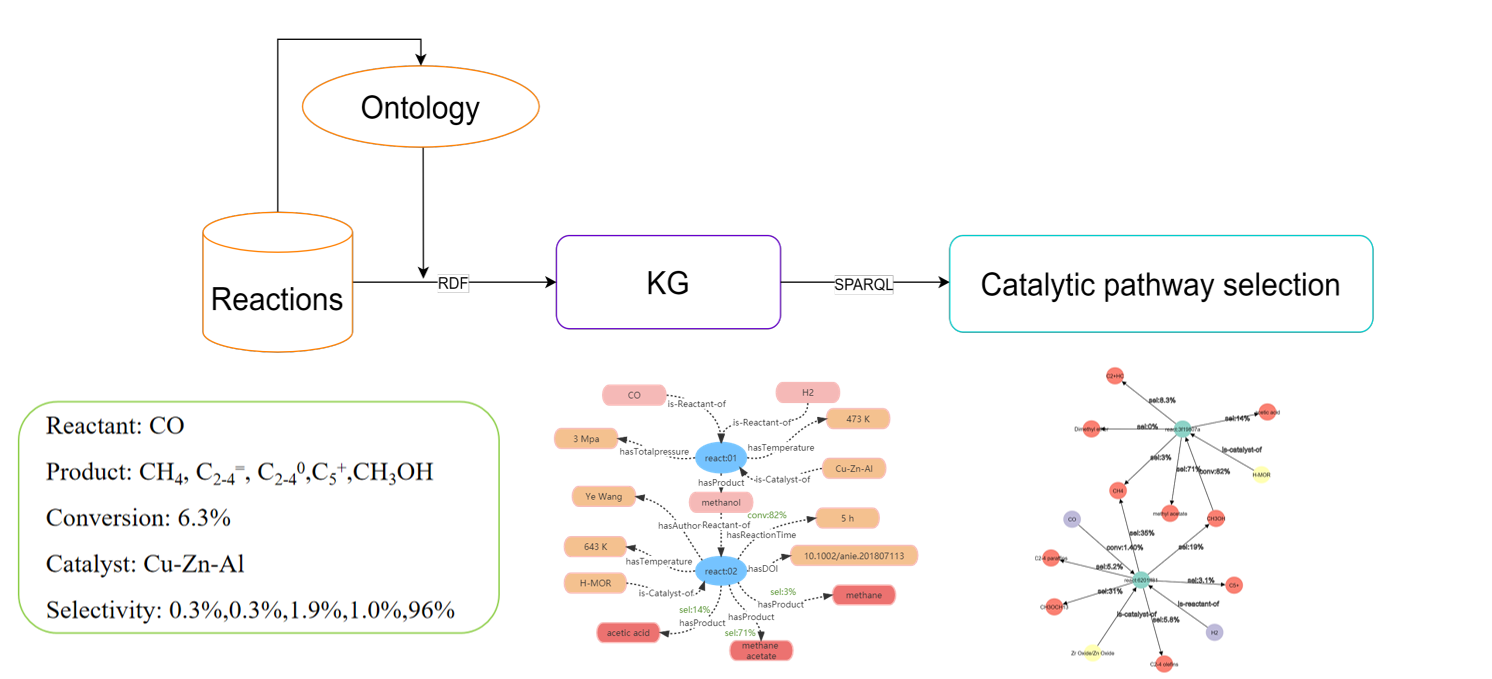
\includegraphics[width=0.7\textwidth]{figure/20.png}
 \caption{ Reactions to knowledge graph }
 \label{ Fig.20 }
\end{figure}

\paragraph{Relay-catalysed path screening}A relay-catalyzed pathway is a synthetic process for a specific molecule that needs to conform to the relay-catalysis concept. We constructed relay-catalyzed rules for a specific reaction pathway taken from the knowledge graph to determine whether the current route fits the relay-catalyzed rules. All the paths retrieved from the knowledge graph are scored using the relay catalyzing rule, and finally, all the paths are sorted in descending order of their scores, and the paths with higher scores are the better relay catalyzing paths we expect, as shown in (Fig.\ref{ Fig.21 }).

\begin{figure}[htbp]
 \centering
 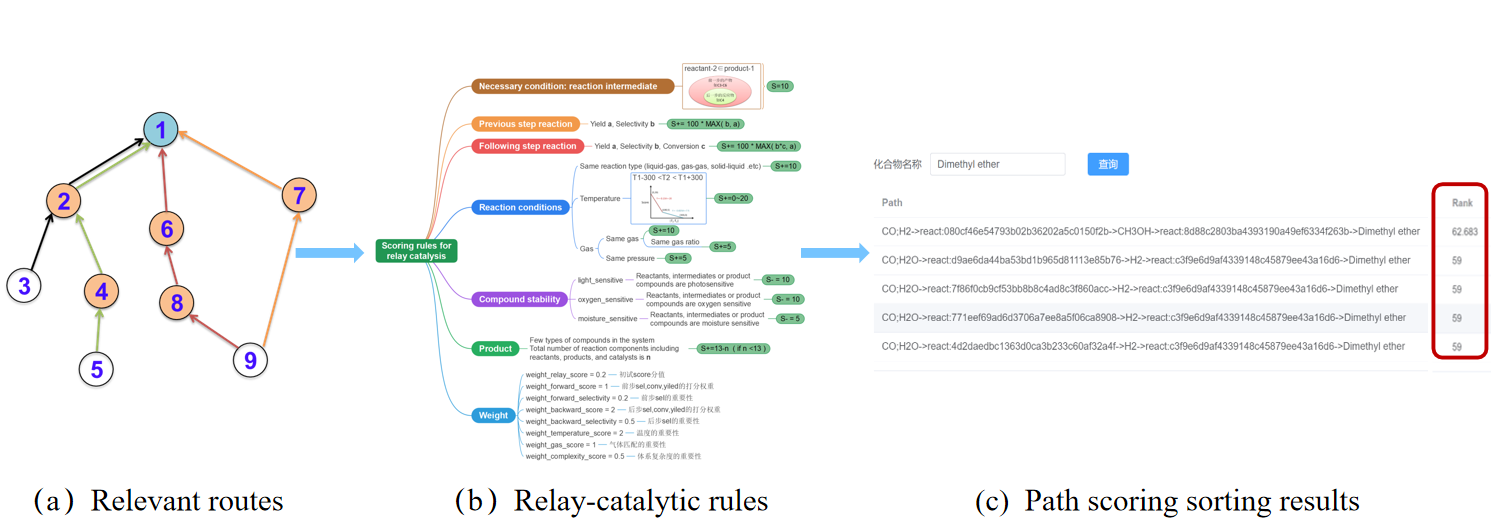
\includegraphics[width=0.7\textwidth]{figure/21.png}
 \caption{ Application of relay catalysis with catalytic knowledge graph }
 \label{ Fig.21 }
\end{figure}

Here we retrieved more than sixty catalytic pathways and their corresponding scores from the knowledge graph as shown in (Fig.\ref{ Fig.22 }), and found that the highest-scoring pathway in the automated screening results was consistent with the relay catalytic pathway reported by Prof. Wang Ye's team; and we also found the second-best-scoring relay catalytic pathway, which was unreported but appeared to be feasible. Here we conclude that it is feasible to automate the screening of relay catalytic pathways using knowledge graph technology, and such a scheme can screen new feasible pathways, which can be used to assist catalytic researchers in exploring new synthetic pathways for compounds.

\begin{figure}[htbp]
    \centering
    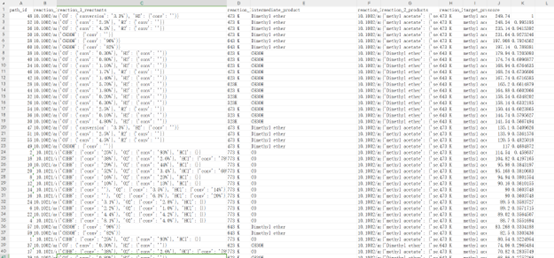
\includegraphics[width=0.7\textwidth]{figure/22.png}
    \caption{ Selected pathways from catalytic knowledge graph }
    \label{ Fig.22 }
   \end{figure}

\section{Opportunities and Challenges}

Knowledge graph-based automatic screening scheme for relay catalytic pathways has been proven to be feasible, but for the application of catalytic knowledge graphs to be able to generalize them, there are still many problems with the current representation of knowledge graphs, such as:

\paragraph{Reaction node representation}It is all the information (reaction conditions, reactants, products, etc.) combined to generate a unique 32-bit string (react:ID), which is not informative, and ID changes if any of the conditions change, not good for searching. We hope to refine the representation of reaction nodes through ontology construction from the perspective of defining a class of reactions in terms of reactants + products.

\paragraph{Catalyst representation}It is all the information of the catalyst (synthesis mode, temperature, precursor) combined to generate a unique 32-bit string (cata:ID). The name itself (e.g. Cu-Zn-Al) does not have a normalized representation, resulting in uninformative catalyst nodes, which is not conducive to the later expansion of catalyst selection and design. We hope to represent specific catalyst nodes in a tree structure from synthesis mode/temperature/precursor.
\paragraph{Compound representation}It is to query the ID corresponding to CHEBI, and those that can be found directly use the ontology information corresponding to CHEBI; compounds that cannot be found use MD5 to encrypt the existing compound name to get a 32-bit string ID (spi:ID), which has two problems:

\begin{itemize}
    \item Compounds that cannot be found use MD5 encrypted strings as IDs
    \item The representation of the compound is not clear enough
\end{itemize}
	

To solve the above problems, we consider that compounds that cannot be found can be uniquely represented by the corresponding CAS number in PubChem. For common mixtures, a separate database of mixtures is constructed IDs are assigned, and subordinate relationships between single substances and mixtures are established.


\section{Conclusions}

To achieve all of the potential of this technology, we intend to engineer and automate the process of catalytic knowledge graph construction to increase the amount of data, as well as automate the data validation module to save manpower, optimize the scoring rules for relay catalytic pathways, and explore applications based on the current knowledge base, such as reaction classification, reaction result prediction, and so on.

\begin{acknowledgments}
We wish to acknowledge the support of Professor Jun Cheng, Slviya Wang and colleagues in the lab, offering suggestions and encouragement.

\end{acknowledgments}

\nocite{*}
\bibliography{report}% Produces the bibliography via BibTeX.

\end{document}
%
% ****** End of file report.tex ******
